% mn2esample.tex
%
% v2.1 released 22nd May 2002 (G. Hutton)
%
% The mnsample.tex file has been amended to highlight
% the proper use of LaTeX2e code with the class file
% and using natbib cross-referencing. These changes
% do not reflect the original paper by A. V. Raveendran.
%
% Previous versions of this sample document were
% compatible with the LaTeX 2.09 style file mn.sty
% v1.2 released 5th September 1994 (M. Reed)
% v1.1 released 18th July 1994
% v1.0 released 28th January 1994

\documentclass[useAMS,usenatbib]{mn2e}
%FAG added header file to contain macros
\include{header}
% If your system does not have the AMS fonts version 2.0 installed, then
% remove the useAMS option.
%
% useAMS allows you to obtain upright Greek characters.
% e.g. \umu, \upi etc.  See the section on "Upright Greek characters" in
% this guide for further information.
%
% If you are using AMS 2.0 fonts, bold math letters/symbols are available
% at a larger range of sizes for NFSS release 1 and 2 (using \boldmath or
% preferably \bmath).
%
% The usenatbib command allows the use of Patrick Daly's natbib.sty for
% cross-referencing.
%
% If you wish to typeset the paper in Times font (if you do not have the
% PostScript Type 1 Computer Modern fonts you will need to do this to get
% smoother fonts in a PDF file) then uncomment the next line
% \usepackage{Times}

%%%%% AUTHORS - PLACE YOUR OWN MACROS HERE %%%%%


%%%%%%%%%%%%%%%%%%%%%%%%%%%%%%%%%%%%%%%%%%%%%%%%

\title[The supernova-regulated ISM - III. Magnetic fields in the multi-phase gas]{The supernova-regulated ISM - III. Magnetic fields in the multi-phase gas}
\author[C. C.~Evirgen, A.~Shukurov, F.A. Gent and A.~Fletcher]{C.C.~Evirgen$^{1}$\thanks{E-mail:
c.c.evirgen@newcastle.ac.uk (CCE); anvar.shukurov@newcastle.ac.uk (AS); 
f.gent@shef.ac.uk (FAG); andrew.fletcher@newcastle.ac.uk (AF)}, A.~Shukurov$^{1}$, F.A.~Gent$^{2}$ and A.~Fletcher$^{1}$.\\
$^{1}$School of Mathematics and Statistics, Newcastle University,
Newcastle upon Tyne, UK, NE1 7RU\\
$^{2}$SP$^{\,2}$\!RC, School of Mathematics and Statistics, University of Sheffield, 
Sheffield, UK, S3 7RH}
\begin{document}
\newcommand{\bvec}[1]{\boldsymbol{#1}}
\newcommand{\avg}[1]{\left<\bvec{#1}\right>_{l}}
\date{Accepted -. Received -; in original form -}

\pagerange{\pageref{firstpage}--\pageref{lastpage}} \pubyear{2015}

\maketitle

\label{firstpage}

\begin{abstract}
\ldots 
\end{abstract}

\begin{keywords}
\ldots
\end{keywords}

%--------------------------------------------------------------------------------------------------------------
\section{Introduction}
%--------------------------------------------------------------------------------------------------------------

FAG -- notes -- include Beck, Fletcher, Berkhuijsen observations of magnetic 
fields \citep{BAH13, MNR18065} and observation/estimates of multiphase structure 
\citep{CS74,MO77}

The results presented in this paper are based on simulations of the multiphase 
interstellar medium (ISM) reported in \citet{GSFSM13} and \citet{GSSFM13}, 
subsequently referred to as \HD\, and \MHD, respectively.

In particular we consider a model, identified as B1$\Omega$s in \MHD.
Supernova(SN)-driven turbulence is applied to ISM in a section of a spiral
galaxy differentially rotating, stratified about the galactic disk and subject
to, radiative cooling \citep{Sarazin87,Wolfire95}, photoelectric heating
\citep{Wolfire95} and other transport processes.

The rate and distribution of SN explosions, gravity \citep{Kuijken89} and 
angular momentum are consistent with observational parameters for the solar neighbourhood \citep{F01}. A nano Gauss seed magnetic field is applied and amplified by dynamo until it saturates with a mean magnetic stength of a few micro Gauss, remarkably consistent with observed estimates for the Milky Way \citep{dummy}.

Models of the magnetized ISM \citep{Heitsch01,M-LBKA05} 
%FAG maybe also include Henley et al 2015 end FAG
have explored the effects of magnetic field on the localized ISM, including the fluctuation dynamo, but without the effects of stratification and the large scale structure induced by the differential rotation of the disk.

Large scale structure in the stratified ISM has been investigated by
\citet{AB05a}, but without differential rotation the dynamo to grow the field to full strength is absent, so an imposed field is applied. 
\citet{Hanasz05,Dobbs08} and \citet{Hanasz09} apply magnetic fields to global disk models, including a dynamo, but due to numerical constraints must limit or exclude vertical stratification and multi-phase gas composition.
\citet{Korpi99a} and \cite{Gressel08} conducted earlier simulations with the same approach as described here, but with lower resolution and higher 
diffusion were unable to follow the dynamo through to saturation.
The advantage of the results from \MHD\ is that the magnetic field produced is not imposed, but evolves dynamically under realistic physical processes governing the formation of the thermo-hydrodynamic structure of the ISM.
From this point of view it is of great value for appreciating the multi-phase structure of the magnetized ISM and for comparison with observation.

Twelve snapshots in the time range, $1.40\Gyr<t<1.67\Gyr$ are used. 
This time range corresponds to the steady-state phase of the system. 
 
In addition, a snapshot at $t=1.4$ Gyr is also presented (Figure \ref{fig:fld_lines}) to illustrate the effect of the hot phase on the magnetic field. This snapshot is chosen because it contains a hot gas structure resembling a superbubble, which has length scale $\mathcal O(10^2)$pc, in all physical dimensions. Further the ISM is well stratified in this snapshot; there are no chimney structures of hot gas propagating throughout the simulation domain. This illustrates the contrast in the characteristics of the mean magnetic field lines between the warm and the hot phases.   

The multi-phase structure is defined in terms of temperature and density. However, an equivalent definition is given in terms of entropy, which has an explicit defintion linking density and temperature \citep{Gent12}. The cold, warm and hot phases are defined by the entropy ranges, $s\leq3.7\cdot10^8$, $3.7\cdot10^8<s<23.2\cdot10^8$ and $s>23.2\cdot10^8$ erg g$^{-1}$ K$^{-1}$, respectively. 

%--------------------------------------------------------------------------------------------------------------
\section{The mean magnetic field}
%--------------------------------------------------------------------------------------------------------------
The decomposition of the magnetic field into mean and fluctuating (random) field follows \MHD.

Volume averaging with a Gaussian kernel, $G_{l}(\bvec{x}-\bvec{x}')$ is used to decompose the magnetic field, $\bvec{B}$, into mean (large-scale), $\bvec{B}_{l}$ and random (small-scale), $\bvec{b}_{l}$, fields. The decomposition is given by 
\begin{equation}
\bvec{B} = \bvec{B}_{l}+\bvec{b}_{l},\qquad \bvec{B}_{l} = \avg{B}. \label{decomp} 
\end{equation}
Gaussian smoothing of the magnetic field with kernel size $l$ is represented by
\begin{align}
\avg{B}&=\int_{V}\bvec{B}(\bvec{x}')G_{l}(\bvec{x}-\bvec{x}')d^{3}\bvec{x}',\\
G_{l}(\bvec{x})&=(2\pi l^2)^{-3/2}\exp[-\bvec{x}/(2l^2)],\nonumber
\label{gauss}
\end{align} 
where $l\approx50$pc is half the integral scale of random motions, as discussed
in \HD.  

Preliminary analysis does not show significant sensitivity of the mean or random field to variations in $l$ within the range $30<l<100$pc. However, future work will consider analysis of isolated structures in the ISM. A more detailed analysis of length and correlation scales will be carried out. However, the current definition, $l=50$pc, is sufficient for the purposes of this paper. 
%--------------------------------------------------------------------------------------------------------------
\section{Three-phase structure of the Field}\label{sect:3BB}
%--------------------------------------------------------------------------------------------------------------         
The total volume probability distributions for gas number density $n$, temperature $T$ and thermal pressure $p$ are displayed in Fig.~\ref{fig:pdfm} from Models~$\Ompa$ (black, solid) and $\Omph$ (blue, dashed). Note that Model~$\Omph$ includes the correction to the SN distribution, which stabilises the disc against unphysical cyclic oscillations, although it is still subject to natural random vertical fluctuations. Hence the mean density in the SN active region remains consistently higher than in Model~\Op.
%--------------------------------------------------------------------------------------------------------------
  \begin{figure}
  \centering\hspace{-2cm}
  \includegraphics[width=0.36\columnwidth,clip=true,trim=0 0 0 9mm]{fig/o1pr_rpdf.png}
  \includegraphics[width=0.36\columnwidth,clip=true,trim=0 0 0 9mm]{fig/o1pr_tpdf.png}
  \includegraphics[width=0.36\columnwidth,clip=true,trim=0 0 0 9mm]{fig/o1pr_ppdf.png}
  \hspace{-2cm}
    \caption[Total volume probability distributions for Model~$\Ompa$ and $\Omph$]{
  Volume weighted probability distributions of gas number
  density~{\textbf{(a)}}, temperature~{\textbf{(b)}} and thermal
  pressure~{\textbf{(c)}} for  models {$\Omph$} (black, solid) and
  {$\Ompa$} (blue, dashed) for the total numerical domain $|z|\le1.12\kpc$.
    \label{fig:pdfm}}
  \end{figure}
%--------------------------------------------------------------------------------------------------------------

Although the three phase temperature distribution is still visible for this model in Fig.~\ref{fig:pdfm}b, it is less pronounced than the results from Model~\Op\ shown in Fig.~\ref{fig:pdf2}b. However the three phase structure for the MHD Model~$\Ompa$ is not at all apparent in panel b, with a significantly narrower range of temperatures. The bulk of the density distributions (a) are quite similar between the HD and MHD models, except that the high densities are not as well resolved in the MHD models. The thermal pressure distributions are very similar, but with the HD modal pressure approximately one third the MHD modal pressure. 

%--------------------------------------------------------------------------------------------------------------
  \begin{figure}
  \centering\hspace{-2cm}
  \includegraphics[width=0.535\columnwidth]{fig/zrhom.png}
  \includegraphics[width=0.535\columnwidth]{fig/zrppm.png}\hspace{-2cm}
    \caption[Horizontal averages of $n$ and $P$ for Model~$\Ompa$ and $\Omph$]{
  Horizontal averages of gas number density, $\mean{n}(z)$ {\textbf{(a)}}, and
  total pressure, $\mean{P}(z)$ {\textbf{(b)}}, for Model~{$\Ompa$} (solid,
  black), and Model~{$\Omph$} (dashed, blue). 
  Each are time-averaged using eleven snapshots respectively, spanning 
  100\Myr.
  The vertical lines indicate standard deviation within each horizontal slice.
  The thermal $\mean{p}(z)$ (dotted) and ram $\mean{p}\turb(z)$ (fine dashed)
  pressures are also plotted {\textbf{(b)}}.
  For Model~{\OpH} the magnetic pressure $\mean{p}_B$ is also plotted (fine, 
  dash-3dotted).
    \label{fig:zrhom}
            }
  \end{figure}
%--------------------------------------------------------------------------------------------------------------

The effect of the magnetic pressure in Model~$\Ompa$ is to expand the thick disc further than Model~$\Omph$ and this is illustrated in Fig.~\ref{fig:zrhom}a, where the horizontal averages of gas number density $n(z)$ are plotted against $z$ for both models. The strong peak in the density at the mid-plane is evident for Model~$\Omph$ (black, solid), while for Model~$\Ompa$ (blue, dashed) there is a broad plateau in the density, extending to $|z|\simeq300\pc$, where the mean magnetic field is strongest.

%--------------------------------------------------------------------------------------------------------------
  \begin{figure}
  \centering
  \includegraphics[width=0.45\linewidth]{fig/o1pr_npdf3s.png}  
  \includegraphics[width=0.45\linewidth]{fig/o1ph_npdf3s.png}\\  
  \includegraphics[width=0.45\linewidth]{fig/o1pr_tpdf3s.png}
  \includegraphics[width=0.45\linewidth]{fig/o1ph_tpdf3s.png}  
    \caption[Probability distributions by phase for $n$ and $T$]{
  Probability distributions by phase: cold (blue, dashed), warm (black, solid)
  and hot (red, dash-dotted) for gas number density ($n$ {\textbf{(a), (b)}})
  and temperature ($T$ {\textbf{(c), (d)}}) 
  for Model~$\Ompa$ ({\textbf{(a), (c)}}) and Model~$\Omph$
  ({\textbf{(b), (d)}}). 
  95\% confidence intervals for temporal deviation are shown as error bars.   
  \label{fig:npdf3s}
    }
  \end{figure}
%--------------------------------------------------------------------------------------------------------------

The horizontal averages of the pressure are plotted in Fig.~\ref{fig:zrhom}b for both models. There is a strong peak at the mid-plane in the turbulent pressure for the HD model (black, dashed), but a much weaker profile for the MHD model (blue, dash-dotted). There are two peaks in the magnetic pressure (blue, dash-3dotted) near $|z|\simeq200\pc$, which supports the extended density profile. Another possible effect, which might constrain the circulation of the hot gas, and hence enhance the pressure at the mid-plane, is the strong horizontal orientation of the field.

As mentioned in Section~$7.2$ in \citet{Gent12} the periodic boundary conditions exclude a non-zero vertical component to the mean field, so the magnetic tension predominantly acts against the vertical flows. Some understanding of the multi-phase structure of the magnetised ISM is still possible from these models, but the extreme temperatures and densities
are significantly under represented.

To improve this in future work it will be desirable to allow unrestricted  evolution of vertical field and to apply realistic clustering of the SNe to generate more supperbubbles (composite multiple SN remnants forming a  single superstructure) or chimneys (plumes venting hot gas from the disc  towards the halo).

Results for separation of the ISM into three phases using the method  detailed in Section~\ref{sect:entropy} are shown for Models~$\Ompa$ and  $\Omph$ in Fig~\ref{fig:npdf3s} with total volume probability distributions.
The phases are defined using entropy $s$ such that for cold  $s<4.4\cdot10^{8}\erg \g^{-1}\K^{-1}$ and hot $s>23.2\cdot10^{8}\erg \g^{-1}\K^{-1}$ with warm in between.
Apart from the higher densities for the cold phase with the HD model (panel b), anticipated by the volume distributions (Fig.~\ref{fig:pdfm}), the warm and hot distributions for the MHD density (panel a) are broad, with a bimodal structure to the hot gas. 
The distributions for the warm gas (panels c and d) are very similar and for the cold (hot) distributions the MHD model does not extend to as low (high) temperatures. 

%--------------------------------------------------------------------------------------------------------------
  \begin{figure}
  \centering
  \includegraphics[width=0.475\linewidth]{fig/o1pr_pdf2dtn.png}  
  \includegraphics[width=0.475\linewidth]{fig/o1ph_pdf2dtn.png}
    \caption[2D probability distribution of $n$ and $T$ for Models~$\Ompa$ and $\Omph$]{
  Probability contour plot by volume of log$n$ vs log$T$ for Model~$\Ompa$
  {\textbf{(a)}}
  and Model~$\Omph$ {\textbf{(b)}}.
  The lines of constant entropy $s=4.4\cdot10^{8}$ 
  and $23.2\cdot10^{8}\erg\g^{-1}\K^{-1}$ indicate where the phases are defined
  as cold for $s\le4.4$ and as hot for $s>23.2$. 
  \label{fig:b2dv}
    }
  \end{figure}
%--------------------------------------------------------------------------------------------------------------

Comparing the combined probability distribution of density and temperature for both of these models in Fig.~\ref{fig:b2dv} with those of Model~\Op\ in Fig.~\ref{fig:pdf2d} the spread is more broad and not obviously aligned along a line of constant pressure.
The HD distribution here is less compact than with MHD.  However when considering only the mid-plane distributions, as displayed in Fig.~\ref{fig:b2dh} the distributions match better with Model~\Op\ and the pressure alignment is evident. So the broad distributions for the total volumes are explained by the stronger gradient in the pressure distribution, due to the reduced stirring of the hot gas.

The thermal pressure at the mid-plane is also very similar in both models,  reflected also in the agreement of the total and thermal pressure near the  mid-plane in the plot of horizontal averages (Fig~\ref{fig:zrhom}b). The magnetic and turbulent pressure in Model~$\Ompa$ combine to match the mid-plane turbulent pressure alone of Model~$\Omph$.
For the temperature in Model~$\Ompa$ the hot gas has two modes, evident in Fig.~\ref{fig:b2dv}a at $10^5\K$ and $10^6\K$, but at the mid-plane there only the single $10^3\K$ mode. The structure of the ISM at the mid-plane is therefore common to both models with modes at $10^6\K,~10^{-2}\cmcube$ and $10^4\K,~1\cmcube$.
The cold gas is insufficiently resolved in Model~$\Ompa$ for comparison.   

%--------------------------------------------------------------------------------------------------------------
  \begin{figure}
  \centering
  \includegraphics[width=0.475\linewidth]{fig/o1pr_pdf2dh.png}  
  \includegraphics[width=0.475\linewidth]{fig/o1ph_pdf2dh.png}
    \caption[2D mid-plane probability distribution for Models~$\Ompa$ and  $\Omph$]{
  The mid-plane probability distributions ($|z|<100\pc$) by gas number density 
  $\log n$ and temperature $\log T$ for {\textbf{(a)}} Model~$\Ompa$ and
  {\textbf{(b)}} Model~$\Omph$.
  \label{fig:b2dh}
    }
  \end{figure}
%--------------------------------------------------------------------------------------------------------------

There is no evident dependence in the probability distributions between the MHD models differing in rotation, shear or SN rate. The models in the kinematic stage extend to lower densities and higher temperatures than either the HD Model~$\Omph$ or the MHD models in the dynamo saturated state, and also extend to lower pressures.

%--------------------------------------------------------------------------------------------------------------
  \begin{figure}
  \centering
  \includegraphics[width=0.475\linewidth]{fig/o1pr_pdf2db.png}  
  \includegraphics[width=0.475\linewidth]{fig/o1pr_pdf2tb.png}
    \caption[2D probability distribution of $n,B$ and $B,T$ for Model~$\Ompa$]{
  Total volume probability distributions ($|z|<100\pc$) by gas number density 
  $\log n$ and magnetic field strength $\log |B|$ {\textbf{(a)}} and
  temperature $\log |T|$ and magnetic field strength $\log |B|$ 
  {\textbf{(b)}} for Model~$\Ompa$.
  \label{fig:b2dnt}
    }
  \end{figure}
%--------------------------------------------------------------------------------------------------------------

In Fig.~\ref{fig:b2dnt}a the joint probability distributions of gas number  density with magnetic field strength is shown and in Fig.~\ref{fig:b2dnt}b  of temperature with magnetic field strength for Model~$\Ompa$. From (a) it is clear there is a strong positive correlation between magnetic field strength and density and from (b) a weak negative correlation between  temperature and field strength. The $T,B$ distribution has very strong peak at $T=10^4\K$.    

%--------------------------------------------------------------------------------------------------------------
  \begin{figure*}
  \centering
  \hspace{-3.5cm}
  %\includegraphics[angle=90, width=0.5\linewidth]{fig/b310h.png}\vspace{-1.15cm}\\
  %\includegraphics[angle=90, width=0.5\linewidth]{fig/b310w.png}\vspace{-1.15cm}\\
  %\includegraphics[angle=90, width=0.5\linewidth]{fig/b310c.png}
  \includegraphics[angle=0, trim=0.5cm 0cm 2cm 0cm, clip=true, totalheight=0.33\textheight]{fig/b310c.png}\hspace{-1.15cm}
  \includegraphics[angle=0, trim=0.5cm 0cm 2cm 0cm, clip=true, totalheight=0.33\textheight]{fig/b310w.png}\hspace{-1.15cm}
  \includegraphics[angle=0, trim=0.5cm 0cm 2cm 0cm, clip=true, totalheight=0.33\textheight]{fig/b310h.png}
  \hspace{-4.5cm}
  \caption[Volume snapshots of $\vect{B}$ by phase for Model~$\Ompa$]{
  Vector plots of the magnetic field $\vect{B}$ {\text{(a)}} in the cold phase
  {\text{(b)}} the warm phase and {\text{(c)}} the hot phase.
  Field directions are indicated by arrows and strength by their thickness.
  The colour of the arrows indicates the strength of the
  azimuthal ($y$) component (colour bar on the right).
  The background shading illustrates the density of the ISM.
  \label{fig:b3box}}
  \end{figure*}
%--------------------------------------------------------------------------------------------------------------

For Model~$\Ompa$ the ISM for a single snapshot is decomposed into the  three phases and the magnetic field for each plotted separately in  Fig.~\ref{fig:b3box}.
In panel a the cold gas occupies only a limited volume near the mid-plane,  but the magnetic field is very strong and organised in alignment with the  mean field surrounding it in the warm gas. This is represented by the length and thickness of the vector arrows. The colour of the arrows emphasises that the alignment has a strong azimuthal component. No arrows are present away from the mid-plane, because the cold gas is absent there.
In panel b the warm gas is present throughout the numerical volume.
Field vectors are present almost throughout and the field is highly aligned, 
mainly in the azimuthal direction. 

The strength of the field increases towards the mid-plane. The presence of some vectors in blue or grey indicates that there are significant perturbations where the field includes reversals, some of these strong.

Some of the field exhibits significant vertical orientation, but it is mainly horizontal.
In panel (c) the hot gas is also present throughout the volume, although in smaller amounts near the mid-plane. Despite this there is very little magnetic field. What field there is generally weak and lacks much systematic alignment, although any orientation tends to be vertical, consistent with the field lines being stretched by the gas flowing away from the mid-plane. Effectively the hot gas has a very weak field, which is highly disordered. Most of the magnetic field, and particularly the mean field, occupies the warm gas.
Detailed quantitative analysis of the structure of the gas will be deferred to future work.

%--------------------------------------------------------------------------------------------------------------
\subsection{Summary}

The magnitude of the magnetic field is strongly aligned to the density of the ISM and indirectly the warm and cold phases. More particularly the mean field is stronger in the warm and cold gas, with the hot gas containing a more random field. The mean magnetic field and the magnetic energy is strongest at $|z|\simeq300\pc$, just outside the SNe active region. 
The fluctuating dynamo is likely to be strongest in this SNe active region, 
but due to the low magnetic Reynolds numbers in the simulations, it is likely that the field and energy is significantly weaker in the simulations than might be expected.

%--------------------------------------------------------------------------------------------------------------
\section[]{Magnetic field lines}
%--------------------------------------------------------------------------------------------------------------

We introduce sampling of physical variables along the field lines of the  magnetic field, to obtain a quantitative description of the observables such as entropy.

Sampling along field lines provides an ensemble average across multiple snapshots, whilst avoiding the use of time averages, which is not 
sensible for observables associated with a turbulent flow \citep{TL72}. 
The mean magnetic field is considered first, which is obtained using Gaussian volume averaging of the magnetic field data from simulations.  

An important feature of the mean magnetic field, strongly suggested by theory but never verified observationally or in numerical simulations, is that it is generated by the turbulent dynamo action in the warm gas \citep{S07}. The cold phase occupies too small a volume to be a host of the global dynamo action. The hot phase is unsteady, with the hot gas leaving the galactic disc for the halo at a time scale shorter than the dynamo time scale.

However, it is difficult to verify this suggestion. Magnetic energy is not suitable for this since most of the gas mass is in the cold phase, which biases the energy distribution very strongly. Enhanced local velocity shear produces a similar bias in the hot phase.

We suggest a new approach to probing the relation of the magnetic field to the multi-phase structure, based on the relative fraction of the magnetic field line length in each phase. The question we are able to address is; do magnetic field lines of the mean field prefer any of the phases? If so, which phase does it prefer? Is there any difference between the mean and random magnetic field lines in this respect?

To answer these questions, we compute the PDFs of specific entropy along magnetic field lines and along straight lines. We expect that any bias of the magnetic field, with respect to the multi-phase structure, will be visible in the PDFs. Moreover, for the straight line sampling the probability of each phase must be equal to its fractional volume, which is easy to calculate by volume averaging. This provides an essential control of the method.   
%--------------------------------------------------------------------------------------------------------------
\subsection{Field line equation for a vector field, $\bvec{B}(\bvec{x})$}
%--------------------------------------------------------------------------------------------------------------
Given a vector field, $\bvec{B}(\bvec{x})$, in Cartesian coordinates, its field lines are described by
\begin{equation}
\frac{dx}{B_{x}}=\frac{dy}{B_{y}}=\frac{dz}{B_{z}}=ds,
\label{f_lines_eqn}
\end{equation}
where $ds$ is a separation constant used to integrate along the field line. This is formulated as
\begin{equation}
\displaystyle
\begin{cases}
\frac{dx}{ds}=B_x,\\
\frac{dy}{ds}=B_y,\\
\frac{dz}{ds}=B_z,
\end{cases}
\label{fld_eqns}
\end{equation}
 The field line equation is integrated along $x$, $y$ and $z$ to obtain the field lines,
\[L: (x(s),y(s),z(s)),\]
which are integrated using a $4^{th}$-order Runge-Kutta scheme. For discrete-valued $\bvec{B}(\bvec{x})$ interpolation is used to evaluate its components at positions, $\bvec{x}$, which do not lie on the data grid.
\subsubsection{Sampling observables along field lines}
Having obtained a set of field lines, observables are sampled on each point along the field lines. The multi-phase structure of the ISM gas and the turbulent flows within the ISM gas suggest that the data obtained from sampling these observables along the field lines will not necessarily have a simple, parametric statistical description. Consequently, the histograms are sensitive to the number and choice of location of bins. We circumvent this issue by using Gaussian kernel density estimation, which provides a non-parametric method for obtaining a probability density function (PDF) of the sampled observable data. In this method, the PDF is calculated by taking a linear combination of Gaussian kernels, each centred at a data point. 

We focus on PDFs of entropy, $s$, sampled along field lines, denoted as $\mathcal{P}(s)$. The definition of the multi-phase structure is given below in terms of specific entropy, $s$, with units erg g$^{-1}$ K$^{-1}$:
%--------------------------------------------------------------------------------------------------------------
\begin{equation}
\begin{cases}
\text{Cold phase:}\qquad s\leq3.7\cdot10^8,\\
\text{Warm phase:}\qquad 3.7\cdot10^8<s\leq23.2\cdot10^8,\\
\text{Hot phase:}\qquad s>23.2\cdot10^8.\\
\end{cases}
\label{phase_defns}
\end{equation} 
%--------------------------------------------------------------------------------------------------------------
We define the probability of finding a point along a field line in each of the phases using the phase definitions. These are
%--------------------------------------------------------------------------------------------------------------
\begin{align}
\mathcal P(\text{cold phase})&\equiv\mathcal P(s\leq3.7\cdot10^8),\nonumber\\
\mathcal P(\text{warm phase})&\equiv\mathcal P(3.7\cdot10^8<s<23.2\cdot10^8),\\
\mathcal P(\text{hot phase})&\equiv\mathcal P(s>23.2\cdot10^8).\nonumber
\end{align}
%--------------------------------------------------------------------------------------------------------------
We make extensive use of PDFs of sampled variables, both graphically and to make specific statements about the characteristics of the magnetic fields in the ISM.
%--------------------------------------------------------------------------------------------------------------
\subsubsection{Sensitivity of magnetic field lines to the multi-phase structure}
%--------------------------------------------------------------------------------------------------------------
The mean field is generally aligned with the azimuthal $(y)$ direction. Thus, we use an idea from the field of stereology, which states that, for a statistically homogeneous random field, samples taken from the entire volume and along arbitrary lines through it are statistically equivalent \citep{BJ04}.

Since we sample specific entropy along mean field lines, we can clarify the sensitivity of the mean magnetic field to the multi-phase structure, through a statistical comparison of the samples of entropy along straight lines and mean field lines. The straight lines are launched in the azimuthal direction, from the seed points used to calculate the mean field lines. The straight lines retain the statistical properties of the multi-phase ISM and are aligned in the same direction as the mean field lines. Thus, we should only observe a difference in PDFs of entropy, if mean field lines are sensitive to the multi-phase structure. 

In addition, samples of entropy from snapshots can be combined to form an ensemble average which isolates data pertaining to individual phases of the ISM, without the loss of information expected from time averaging alone. The twelve snapshots used in this paper are statistically independent in time and are taken from the statistically-steady phase of the system.
%\subsubsection{Correlation analysis of magnetic field lines using PDFs}
%We also use PDFs to analyse the correlation lengths of the magnetic fields in the multi-phase. We calculate the maximum displacement of the field lines from their seed point, $r$, and their maximum displacement along the $x$, $y$ and $z$ axes, $r_x$, $r_y$ and $r_z$, respectively. PDFs of these quantities are calculated using kernel density estimation. As an example, we consider some field line, $L_i$, with seed point, $\bvec{x}_0\equiv(x_0,y_0,z_0)$. The field line must have a minimum and maximum displacement from the seed point, which is a direct consequence of the solenoidality of the magnetic field. The maximum displacement occurs at some $\bvec{x}_{max}$ along $L_i$ such that $r=|\bvec{x_{max}}-\bvec{x}|$. The maximum displacements along the axes are described by $r_x = x_{max}-x_0$, $r_y = y_{max}-y_0$, $r_z = z_{max}-z_0$. We calculate typical length scales for each of these displacements, using the mean of the random variable. For example, for $r$, we use
%\begin{equation}
%C = \int_{r_{min}}^{r_{max}}r\mathcal{P}(r)dr,
%\end{equation}
%where $r_{min}$ and $r_{max}$ are the minimum and maximum values of $r$ observed across all snapshots and $\mathcal{P}(r)$ is the PDF of $r$. The typical length scales $C_x$, $C_y$, $C_z$ along the $x$, $y$ and $z$ axes, respectively, are calculated using similar expressions.
%-------------------------------------------------------------------------------------------------------------- 
\subsection{The phase that hosts the magnetic field}
%--------------------------------------------------------------------------------------------------------------
\subsubsection{Distortion of the mean magnetic field lines in the hot phase}
%--------------------------------------------------------------------------------------------------------------
The mean magnetic field lines are calculated as described in Eq.~\eqref{fld_eqns} and a $3$D visualisation is given in Fig.~\ref{fig:vis_td}. The white lines in the box represent the mean magnetic field lines. 

Figure~\ref{fig:vis_td}(b) makes it especially clear that the ISM gas is stratified, as expected from the ISM in the galactic disk. The yellow shades represent the warm phase and the darker, red shades represent the hotter, less dense hot phase. The mean field lines are generally aligned in the azimuthal ($y$) direction and mostly span the box along the $y$-axis. We can see in panels (a) and (b) that, in the warm phase, the displacements of the ffield lines in the $x$ and $z$ directions are much smaller those along the $y$ direction. On the other hand, distortions of the field lines in the hot gas are rather strong.  

%The the turbulent flows in the $0.6<|z|<1.0$kpc region will have the highest kinetic energies throughout the ISM. Conversely, the magnetic field is very weak in the hot phase (Fig.~\ref{fig:b2dnt}). Subsequently, the kinetic energy of the flows should be at least of a comparable order to the magnetic field energy in this region.  We expect this to cause distortions in the magnetic field (CCE: REFERENCE TAYLOR HERE). The lack of alignment and weakness of the magnetic field in this region (Fig. \ref{fig:b3box}) imply that the magnetic field is sensitive to the hot phase. The characteristics of the magnetic field lines further clarify the effect of the hot phase on the magnetic field.
%--------------------------------------------------------------------------------------------------------------
\begin{sidewaysfigure*}
\centering
\vspace{-17.5cm}
\subfigure[]{\includegraphics[scale=0.34]{fig/snapshot0.png}}
%\hspace{10cm}
\subfigure[]{\includegraphics[scale=0.34]{fig/snapshot0x.png}}
%\hspace{10cm}
\subfigure[]{\includegraphics[scale=0.34]{fig/snapshot0y.png}}
\caption{$3$D rendering of mean magnetic field lines (white lines) in the simulated ISM gas $1.4$~Gyr after the start of the simulation, with gas density colour coded. Panel \textbf{(a)} gives an isometric view, whilst panels \textbf{(b)} and \textbf{(c)} give a view along the $x$ and $y$ axes, respectively.}
\label{fig:vis_td}
\end{sidewaysfigure*}
%--------------------------------------------------------------------------------------------------------------
There is a hot gas bubble clearly visible in panel (c) in the range $0.7<z<1$~kpc, where the mean field lines are wrapped around it. This suggests that the hot gas, which typically exhibits transonic turbulence, has sufficient kinetic energy to distort the magnetic field lines as it expands and travels out of the box. Further, we note a column of hot gas spanning the $z$ axis in the box, in the corner $(y = -0.5~\mathrm{kpc},x = 0.5~\mathrm{kpc})$. We note that the field lines are distorted to avoid entering the hot column. Since SNe typically occur within $0.1$~kpc of the galactic midplane \citep{Gent12}, turbulent kinetic energy is injected into the ISM close to the midplane. If multiple SNe occur close to each other, they can join to form a superbubble producing a chimney-like structure \citep{Gent12} similar to the column observed in Fig.~\ref{fig:vis_td}. The fractional volume of the cold phase is less than $0.01$ \citep{Gent12}, so it is hardly visible in this representation. The fractional volume of the warm phase, $f_{\mathrm{v,warm}}$ is generally between $0.88$ and $0.96$ in the midplane and the fractional volume of the hot phase, $f_{\mathrm{v,hot}}$, is generally between $0.04$ and $0.12$, once the numerical model has reached the statistically steady phase. Hence, we expect the statistical properties of the warm phase to dominate the statistical properties of the ISM.

The sampled specific entropy data from the the field lines and straight lines, from the snapshot at $t=1.4$~Gyr, are used to derive PDFs of specific entropy, $s$, for straight lines and mean field lines shown in Fig, \ref{fig:res_pdf0}. The warm-hot phase boundary is represented by a solid black vertical line in Fig.~\ref{fig:res_pdf0}. 
The probabilities of the mean field lines and straight lines being found in each phase, for the snapshot at $t=1.4$~Gyr, are reported in Table \ref{tab:pdf0_probs}. The mean field lines have a higher probability of passing through the warm phase than straight lines, regardless of the $z$ range in consideration. This result is also obtained for the probabilities calculated after ensemble averaging. In addition, the sampling along straight lines consistently calculates probabilities matching the fractional volumes of the phases, as expected.
%--------------------------------------------------------------------------------------------------------------
\begin{figure}
  \centering 
  \includegraphics[width=\linewidth]{fig/all0.pdf}
  \caption{PDFs of entropy sampled along field lines (blue) and straight lines (red).}
  \label{fig:res_pdf0}
\end{figure} 
%--------------------------------------------------------------------------------------------------------------
At $t=1.4$~Gyr, the PDF of $s$ along the mean field lines, hereafter referred to as \meanprs, has higher probability density in the cooler, denser regions ($3.7~\text{erg g}^{-1}~\text{K}^{-1}<s<15~\text{erg g}^{-1}~\text{K}^{-1}$) of the warm phase. The PDF of $s$ along straight lines, hereafter referred to as \stprs, is higher than \meanprs in the hotter, more turbulent ($s>1.5\cdot10^9$~erg g$^{-1}$ K$^{-1}$) regions of the multi-phase. 

Moreover, we note that \stprs extends to higher $s$ in the hot phase; whilst the maximum entropy observed along mean field lines is approximately $s = 3.1\cdot10^9$ erg g$^{-1}$ K$^{-1}$ the maximum entropy observed along straight lines is $s = 3.5\cdot10^9$ erg g$^{-1}$ K$^{-1}$. In a bubble or other cluster of hot gas, we typically expect the higher entropies to be observed inside the cluster, whereas lower entropies would be observed close to the boundary of the cluster due to optically thin cooling of the gas bubble at the boundary of the bubble.
The mean magnetic field lines reside in the cooler regions of the warm phase. The distortions of the mean field lines featured in the hot phase, especially around SN remnants, renders the hot phase an unsteady environment for the global dynamo.   

We previously observed that the mean field lines are wrapped around the clusters of hot gas and do not tend to pass through the clusters, due to the distorting effect of the hot gas cluster on the mean field. On the other hand, straight lines in the azimuthal direction are not sensitive to the multi-phase structure and can pass through the hottest parts of clusters of hot gas. Consequently, the lower maximum $s$ observed along mean field lines suggests that the mean field lines do not pass through the hottest regions of the ISM gas and thus the higher $s$ values are not observed along the mean field lines.
When the mean magnetic field is wrapped around the hot gas moving out of the box, it temporarily resides in a region of higher entropy; this behaviour amounts to forced advection of the mean field with the hot gas. Rather than passing through the hot gas, the mean field lines tend to change shape quite drastically.  
This interaction between the hot phase and the mean magnetic field lines are observed in all snapshots in the statistically-steady state of the model. It has been observed in $3$D renderings of the mean field lines across all other snapshots (omitted in this paper).
%--------------------------------------------------------------------------------------------------------------
\subsection{The mean and random magnetic fields}
%--------------------------------------------------------------------------------------------------------------
We use Equation \eqref{f_lines_eqn} to construct field lines for the random magnetic field using the same method as for field lines of the mean magnetic field. Sampling along these lines (across twelve snapshots) is used to obtain the PDF of entropy, as seen in the previous section for the mean magnetic field. 
%--------------------------------------------------------------------------------------------------------------
\subsubsection{Ensemble averaged characteristics of the mean and random magnetic field lines }
%--------------------------------------------------------------------------------------------------------------
The typical length scale of SN remnants and other hot gas structures propagating through the box is
similar to the typical length scale of mean magnetic field lines. The random magnetic field
represents the fluctuations in the magnetic field, which occur over smaller length scales. 
Therefore, we do not expect the geometry of the random magnetic field lines to be particularly sensitive
to the multi-phase structure. However, the typical strengths of the mean and random magnetic fields should be sensitive 
to the multi-phase structure and distance from the galactic midplane.
We construct a PDF of entropy sampled along random magnetic field lines, denoted by \rnprs which is
presented in Fig.~\ref{fig:tot_pdfs} alongside \meanprs and \stprs sampled across the twelve snapshots available.
The characteristics of \meanprs seen previously are retained in Fig.~\ref{fig:tot_pdfs}, where data from all twelve snapshots have been ensemble averaged. The ensemble averaging decreased the error of the PDF and shows that the mean field is consistently sensitive to the multi-phase ISM. 
We formulate a two-sample Kolmogorov-Smirnov test for non-parametric distributions as $H_0:$  \stprs $=$ \meanprs against $H_1:$\stprs $\neq$\meanprs. This test is significant to a $1\%$  level, which suggests that we can reject the null hypothesis that \meanprs and \stprs come from the same distribution. The same result is also recovered using a two-sample T-test for two independent samples. This indicates a sensitivity of the mean field to multi-phase structure of the ISM. 
%--------------------------------------------------------------------------------------------------------------
\begin{figure}[h!]
\includegraphics[width=\linewidth]{fig/allall_wrn.pdf}
\caption{PDFs of $s$ along field lines of the mean (blue solid), total (red solid) and random (green solid) magnetic fields. The boundaries of between the cold and warm phases (black dashed) and between the warm and hot phases (black solid) are indicated.}
\label{fig:tot_pdfs}
\end{figure}
%--------------------------------------------------------------------------------------------------------------
%--------------------------------------------------------------------------------------------------------------
\section{Supernova remnants}\label{sec:sn_rem}
%--------------------------------------------------------------------------------------------------------------
An SN remnant is identified in the $0.7<z<0.9$~kpc region of the box at $t=1.4$~Gyr. A horizontal slice of the box is taken at $z=0.798$~kpc, which captures a slice through the SN remnant. We then look at colourmap images of various physical variables with integral lines of $(B_x,B_y)$ overlaid. 
%--------------------------------------------------------------------------------------------------------------
\subsection{Thermal pressure in SN remnants}
%--------------------------------------------------------------------------------------------------------------
Figure~\ref{fig:thp_800} shows the colour map image of logarithmic thermal pressure, $\log(p)$, on the horizontal slice taken at $z=0.798$~kpc at $t=1.4$~Gyr. Integral lines of the horizontal mean magnetic field are overlaid with the colour of the integral lines representing mean magnetic field energy.
%--------------------------------------------------------------------------------------------------------------
\begin{figure}
%\centering
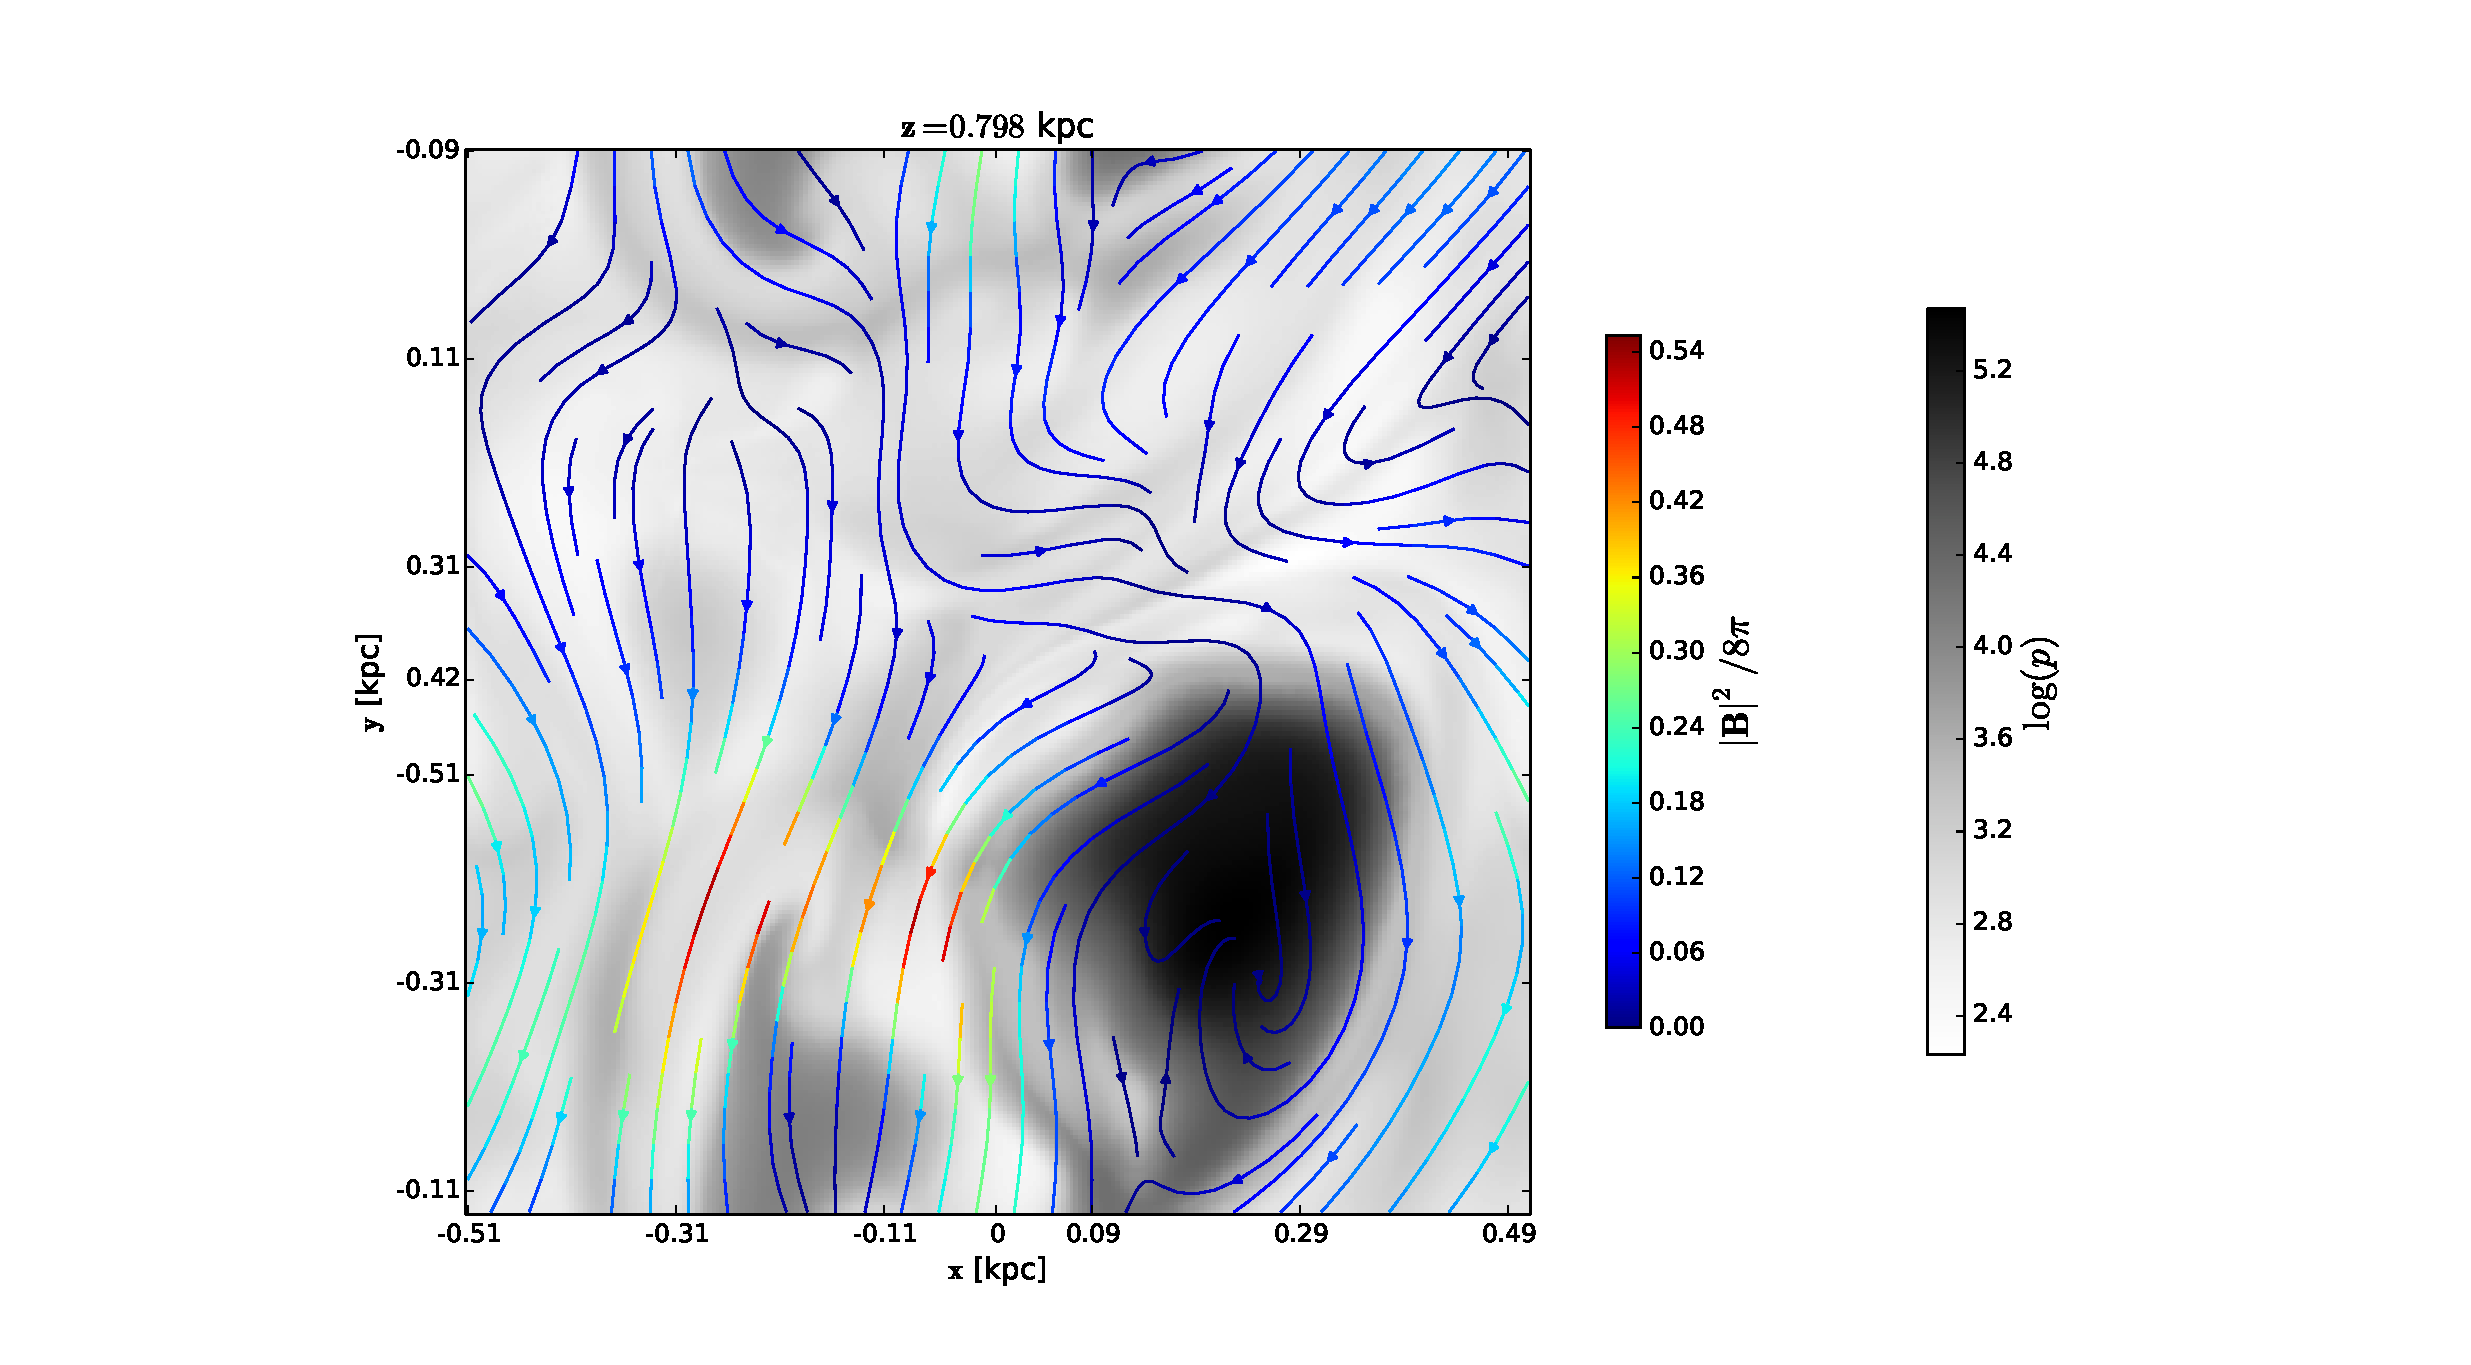
\includegraphics[width = \linewidth]{fig/pp_slice_800pc.eps}
\caption{Thermal pressure (colour coded) with integral lines the horizontal magnetic field at $z=0.798$~kpc.}
\label{fig:thp_800}
\end{figure}
%--------------------------------------------------------------------------------------------------------------
Thermal pressure is used to identify the SN remnant, with extremely high thermal pressures observed inside the SN remnant and a high pressure gradient at the boundaries of the SN remnant. We observe this structure in the bottom right corner of the image. The thermal pressures observed at this slice are typical of the warm and hot phases and we observe values over three orders of magnitude. The highest pressures are observed at the center of the SN remnant. We note that, whilst the pressure is high along the boundary, it is noticeably lower than the pressure at the center. In general, the mean magnetic field is very weak across the slice; it is very weak inside the SN remnant. In addition, we observe that the magnetic field lines generally span the slice in the azimuthal ($y$) direction, forming long structures.

Moreover, the left half of the box is largely unaffected by the SN remnant. Consequently, the mean field integral lines are straighter and less distorted. Conversely, the mean field lines near the SN remnant are wrapped around it. In the right half of the image, we notice that the mean field integral lines still span the slice in the $y$-axis. Yet, they are more perturbed than the lines in the left half, due to the distortions caused by the SN remnant. The correlation of points along the magnetic field implies that the distortions caused in a particular region of the magnetic field can affect the magnetic field structures at large distance, presumably due to magnetic tension.  
%--------------------------------------------------------------------------------------------------------------
\subsection{Gas velocity magnitude in SN remnants}
%--------------------------------------------------------------------------------------------------------------
Figure~\ref{fig:uu_800} shows the gas velocity, $|\bvec{u}|^2$, in the horizontal slice at $z=0.798$~kpc, $t=1.4$~Gyr. Integral lines of the mean horizontal magnetic field are overlaid with the colour of the integral lines representing specific entropy.
%--------------------------------------------------------------------------------------------------------------
\begin{figure}
%\centering
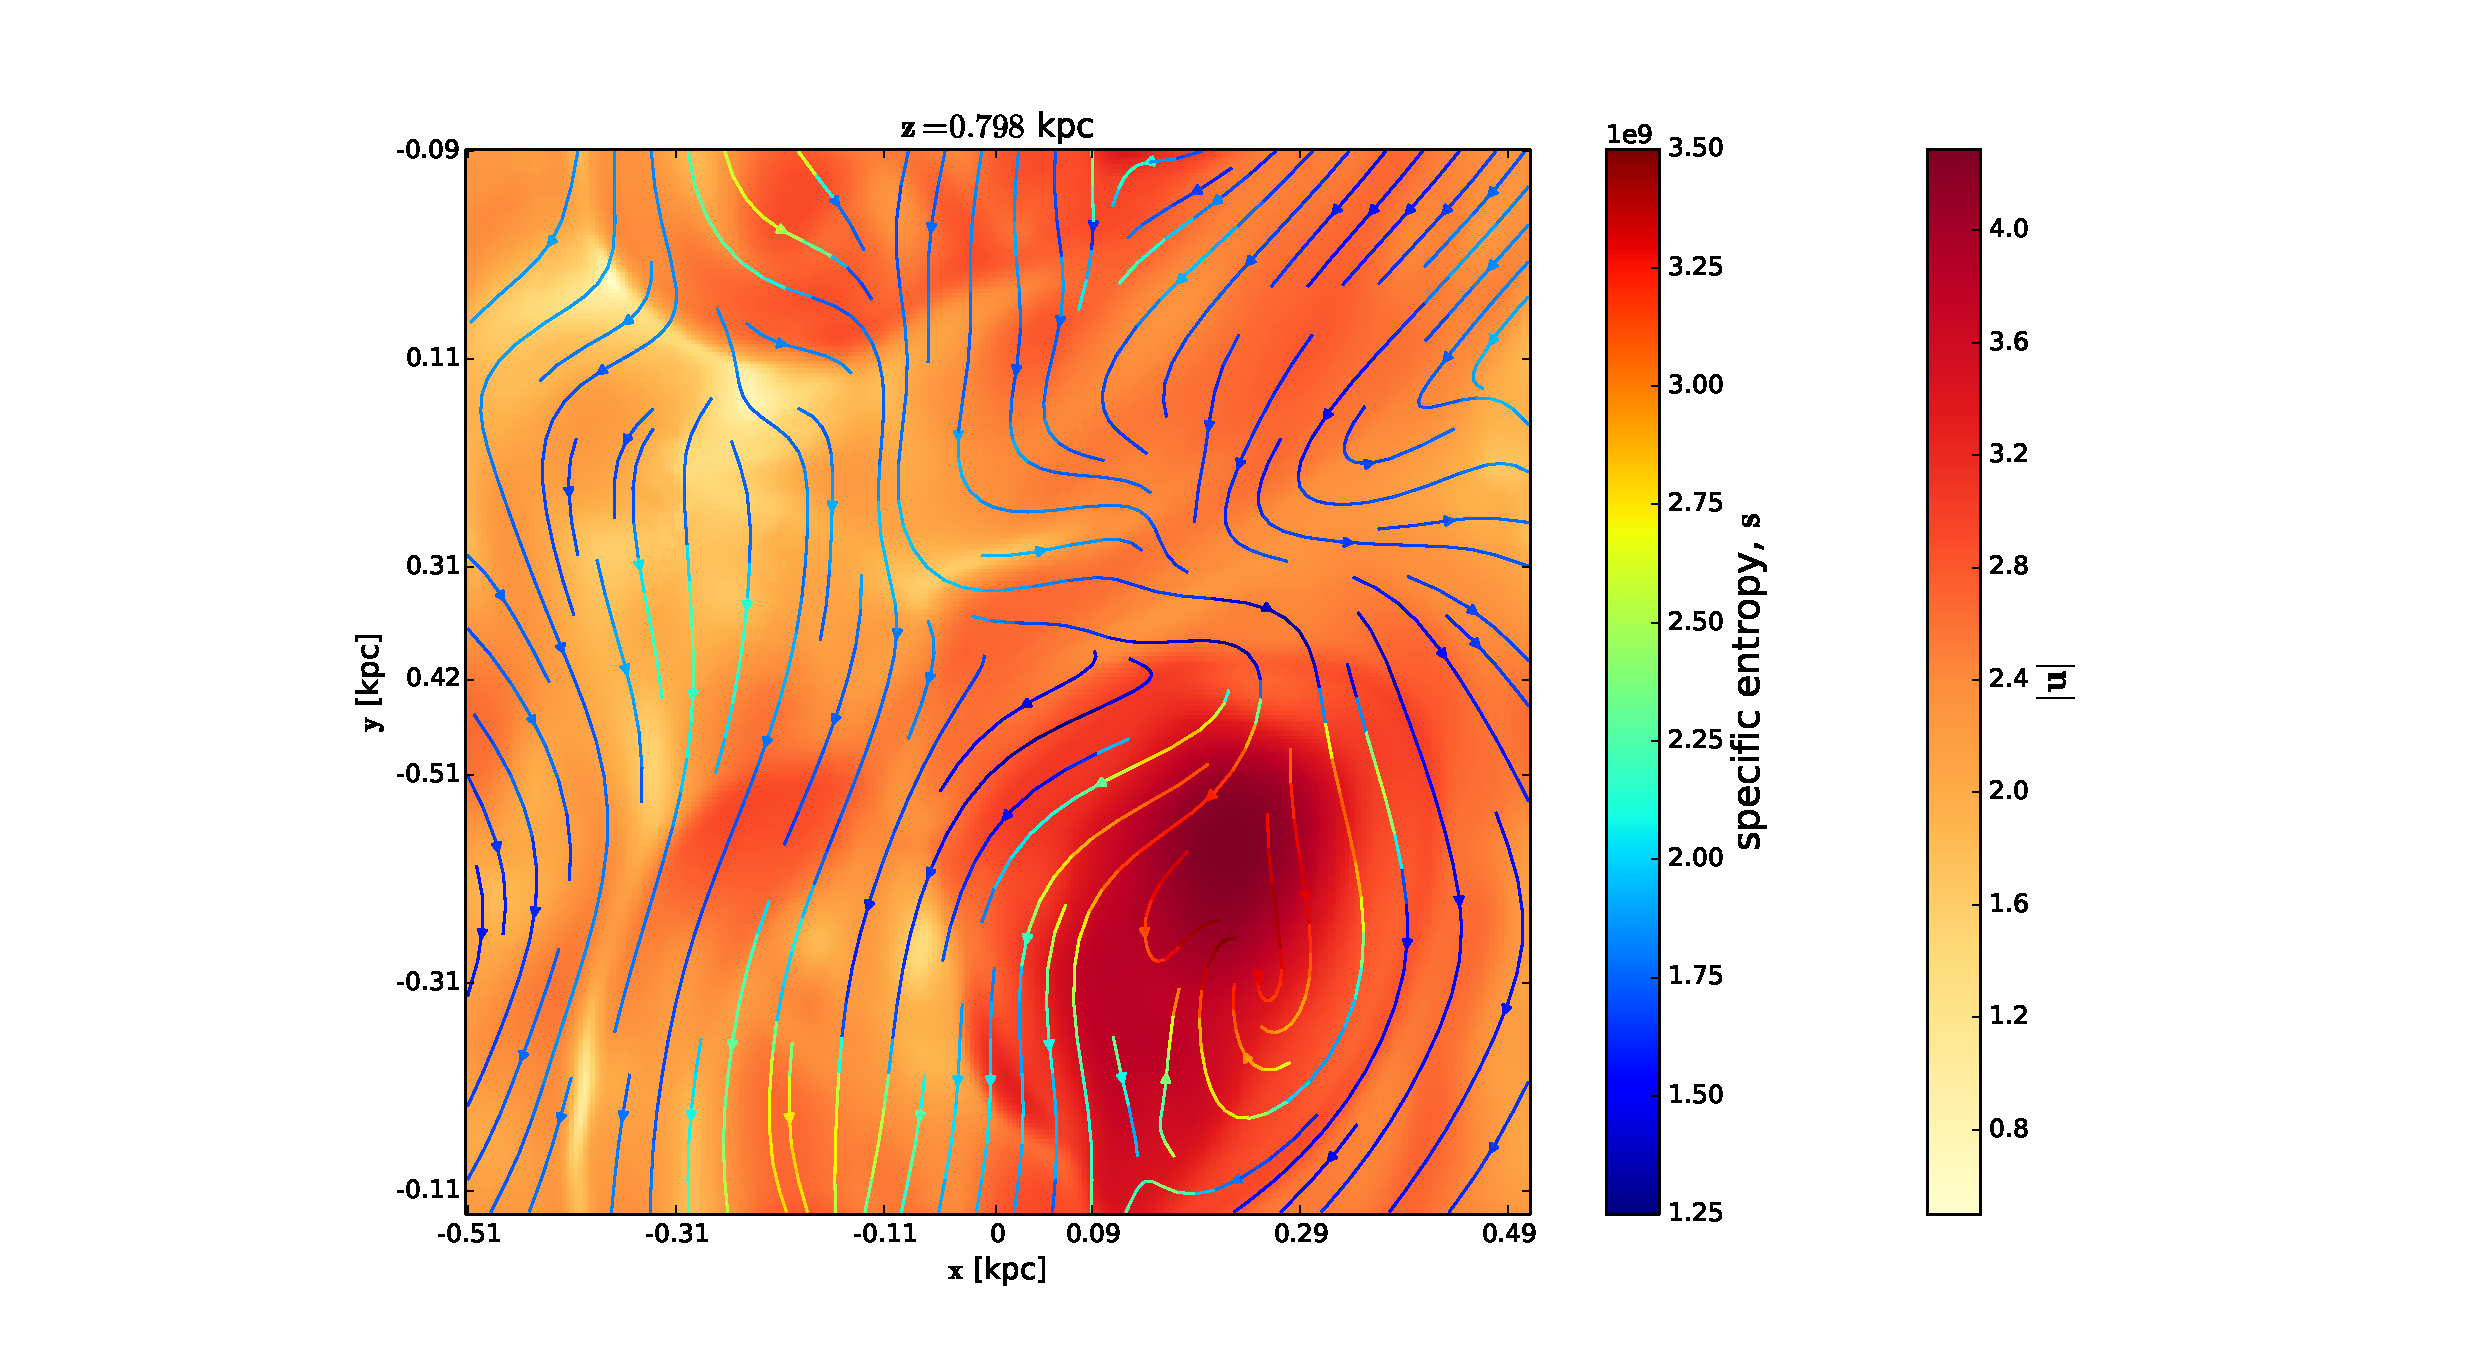
\includegraphics[width = \linewidth]{fig/uu_slice_800pc.eps}
\caption{Gas velocity magnitude with integral lines of $(B_x,B_y)$ at $z=0.798$~kpc, $t=1.4$~Gyr.}
\label{fig:uu_800}
\end{figure}
%--------------------------------------------------------------------------------------------------------------
Both the highest velocities and entropies are observed near the center of the SN remnant. The highest specific entropy, $s\approx3.5\cdot10^9$ erg~g$^{-1}$~K$^{-1}$, corresponds to the maximum specific entropy observed along the straight line in Fig.~\ref{fig:res_pdf0}. The maximum entropy close to the boundary of the SN remnant, $s\approx3.1\cdot10^9$ erg~g$^{-1}$~K$^{-1}$, corresponds to the maximum entropy that \meanprs extends to in the hot phase in Fig.~\ref{fig:res_pdf0}. 

The SN remnant is characterised by high kinetic energy, high entropy and low density. The high pressure gradients across the boundary of the SN remnant and its buoyancy cause the rapid outflows of hot gas, which explains the complete dominance of the hot phase at $|z|>2.5$~kpc region.  

We now consider the PDFs entropy along the field lines and straight lines 
in Figure \ref{fig:pdfs_mean}. 
Firstly, we observe similar peaks in the warm phase. This agrees with Figure \ref{fig:fld_lines} in that the field lines are not sensitive to the warm phase. The probabilities of traversing the phases, for the field lines and straight lines, are given in Table \ref{table:mean_probs}. 
We observe that the probabilities of the straight lines traversing each phase closely match the fractional volumes of the phases, as expected; lines that are not phase-sensitive should traverse each phase with probability proportional to the fractional volume. 

On the other hand, the probability of a field line traversing the hot phase
is significantly higher than that of a straight line, which reiterates the 
effect of the stretching of field lines by the phase. 
The probability of a field line traversing the warm phase is lower than that 
of a straight line. 
However, this is a direct consequence of the distortion of the magnetic field by the hot phase. 
The probability of the field line crossing the cold phase is much smaller than $1\%$ for both field lines and straight lines. The fractional volume of the cold phase is typically very small. Consequently, a different approach is required to analyse the characteristics of the magnetic field in the cold phase.

Overall, the magnetic field lines traverse the ISM in the azimuthal direction. This trend is observed clearly in the warm phase, where the magnetic field is not distorted by the flows of the ISM gas. Since the field lines represent lines of magnetic flux density, the distortion of the magnetic field lines by the hot phase explains the weakness of the magnetic field observed in the hot phase. The stretching of the magnetic field lines effectively wrap the field lines around the hot gas, which increases the field line density on the boundary of the hot and warm gas. 
Consequently, field lines do not pass through the hot gas  (Fig.~\ref{fig:fld_lines}) and we observe that the magnetic field in the hot 
phase is very weak and lacking alignment. 
This strongly suggests that the magnetic field resides in the warm phase.    
%--------------------------------------------------------------------------------------------------------------
\begin{table*}
\centering
\caption{Probabilities of mean field lines and straight lines being found in each phase, calculated in different ranges of $z$.}
\label{tab:pdf0_probs}
\begin{tabular}{lllllll}
      & \multicolumn{2}{l}{Whole box} & \multicolumn{2}{l}{$|z|<0.75$~kpc} & \multicolumn{2}{l}{$|z|>0.75$~kpc} \\ \cline{2-7} 
Phase & Mean field      & Straight lines        & Mean field         & Straight lines          & Mean field         & Straight lines          \\ \hline\hline
Cold  & $\ll 0.01$    & $\ll 0.01$    & $\ll 0.01$       & $\ll 0.01$      & $\ll 0.01$       & $\ll 0.01$      \\
Warm  & 0.93          & 0.88          & 0.95             & 0.91            & 0.91             & 0.86            \\
Hot   & 0.07          & 0.12          & 0.05             & 0.09            & 0.09             & 0.14            \\ \hline
\end{tabular}
\end{table*}
%--------------------------------------------------------------------------------------------------------------
\section{Conclusions}
%--------------------------------------------------------------------------------------------------------------
%FAG
Note, that the mean magnetic field is strongest in the warm phase and the 
dynamo is strongest in the SN dense region within 500\pc of the midplane. 
These results support the hypothesis that the mean field is closely aligned to the warm phase of the ISM.
The fluctuating magnetic field is present in similar magnitude in all phases.
Note, in the warm phase, away from the midplane the magnetic field has a 
stronger vertical component, even though in these models the periodic boundary
conditions constrain the net $B_z$ to be zero on each horizontal slice. 
Given more open horizontal boundaries, we could anticipate the mean field 
actually to exhibit more vertical structure. 
With higher numerical diffusion required for the hot gas, the fluctuation 
dynamo in this phase may have been relatively suppressed, although the 
Reynolds numbers may have been higher than in the warm gas as both the length
scales and the velocities of the turbulence are tyically higher in the hot gas
than in the warm.
Nevertheless, a higher resolution run would be helpful in assessing how robust
is the alignment of the mean field to the warm phase, and whether the
fluctuating field in the hot phase may yet have relatively greater amplitude
than obtained here.
Given the dominance of the dynamo about the midplane, this may be feasible
without extending the domain vertically.

%end FAG

\newpage
%-----------------------------------------------------------------------------
\section*{Acknowledgements}
%-----------------------------------------------------------------------------
  \bibliographystyle{mn2e}      % basic style, author-year citations
  \bibliography{refs}
% name your BibTeX data base
  \label{lastpage}
%end FAG

\label{lastpage}

\end{document}
